\documentclass[10pt]{book}

% For Chinese characters
\usepackage{CJKutf8}
\newcommand{\chinese}[1]{\begin{CJK}{UTF8}{gbsn}#1\end{CJK}}

% Unicode
\usepackage{fdsymbol}
\usepackage[utf8]{inputenc}


% Plotting, table, and figures
\usepackage{tikz}
\usepackage{float}
\usepackage{array}
\usepackage{multirow}
\usepackage{rotating}
\usepackage{pdflscape}
\usepackage{wrapfig}

\usepackage{graphicx}
\graphicspath{ {./figure} }

% Spaces, quotations
\usepackage{parskip}% spaces between paragraphs
\usepackage{setspace}% spaces between lines
\usepackage{csquotes}% English quotations


% Colors
\usepackage{xcolor}
\usepackage{tcolorbox}
\newcommand{\checkme}[1]{\colorbox{red}{#1}}


% The bib style should be set in the documentclass command.
\usepackage[backend=biber,sorting=none,url=false]{biblatex}
\addbibresource{./src/zzhang_phd-thesis_reference.bib}
\renewcommand*{\bibfont}{\normalfont\scriptsize}% using small fonts for reference


% Multiple subfiles
\usepackage{import}
\usepackage[subpreambles=true]{standalone}


% Paper size
\usepackage{geometry}
\geometry{b5paper,bmargin=2.5cm,tmargin=2.5cm,lmargin=3cm}


% To include the title page
\usepackage{pdfpages}


% Title font size, by package titlesec
\usepackage{titlesec}
\usepackage{titletoc}
\titleformat{\chapter}[display]
{\normalfont\Huge\bfseries}
{\textit{\color{black}CHAPTER \thechapter}}
{5pt}{\huge\color{black}}{}


% Foot and header Style
\usepackage{fancyhdr}
\pagestyle{fancy}
\fancyhf{}
\fancyfoot[LE,RO]{\thepage}


% Watermarks
\usepackage{watermark}
\def \marginwatermark#1#2%
{
  \rightwatermark{
    \put(390,#2){
      \tikz[remember picture,overlay]{
      \filldraw[fill=black!75] (0,0) circle (0.60) node{ \LARGE\color{white}\textbf{#1}} (1.25,1); }
    }
  }
}


% Deal Overfull and Underfull
\usepackage[
  activate={true,nocompatibility},
  final,
  tracking=true,
  kerning=true,
  spacing=true,
  factor=1100,
  stretch=15,
  shrink=15]{microtype}


% Deal with overfull \hbox
\pretolerance=150


% URL
\usepackage{hyperref}
\hypersetup{
  colorlinks=true,
  citecolor=black,
  linkcolor=black,
  filecolor=black,
  urlcolor=black!75
}


% Long table
\usepackage{longtable}


% Customize the figure/table captions
\usepackage{caption}
\captionsetup[figure]{labelfont={bf},name={},labelsep=none,singlelinecheck=false}
\captionsetup[table]{labelfont={bf},name={},labelsep=none,singlelinecheck=false}


% Set the line spacing to 1
\onehalfspacing


% Define a box and its style
% Reference https://texample.net/tikz/examples/boxes-with-text-and-math/
\tikzstyle{termbox} = [draw=black,fill=brown!20,very thick,rectangle,
  rounded corners,inner sep=10pt,inner ysep=20pt]
\tikzstyle{termtitle} = [fill=red!5,text=black]


% Add a blank page
\def\blankpage{
  \clearpage
  \thispagestyle{empty}
  \addtocounter{page}{-1}
  \null
  \clearpage
}


% Main text
\begin{document}


% ----------------------------------------------------------------------------
% Front cover
% ----------------------------------------------------------------------------
% \includepdf[pages=-,landscape=true,fitpaper=false,noautoscale=true]{figure/zzhang_phd-thesis_cover.pdf}


% ----------------------------------------------------------------------------
% Title page
% ----------------------------------------------------------------------------
\import{src/chapters/}{zzhang_phd-thesis_titlepage}


% ----------------------------------------------------------------------------
% RUG Title page
% ----------------------------------------------------------------------------
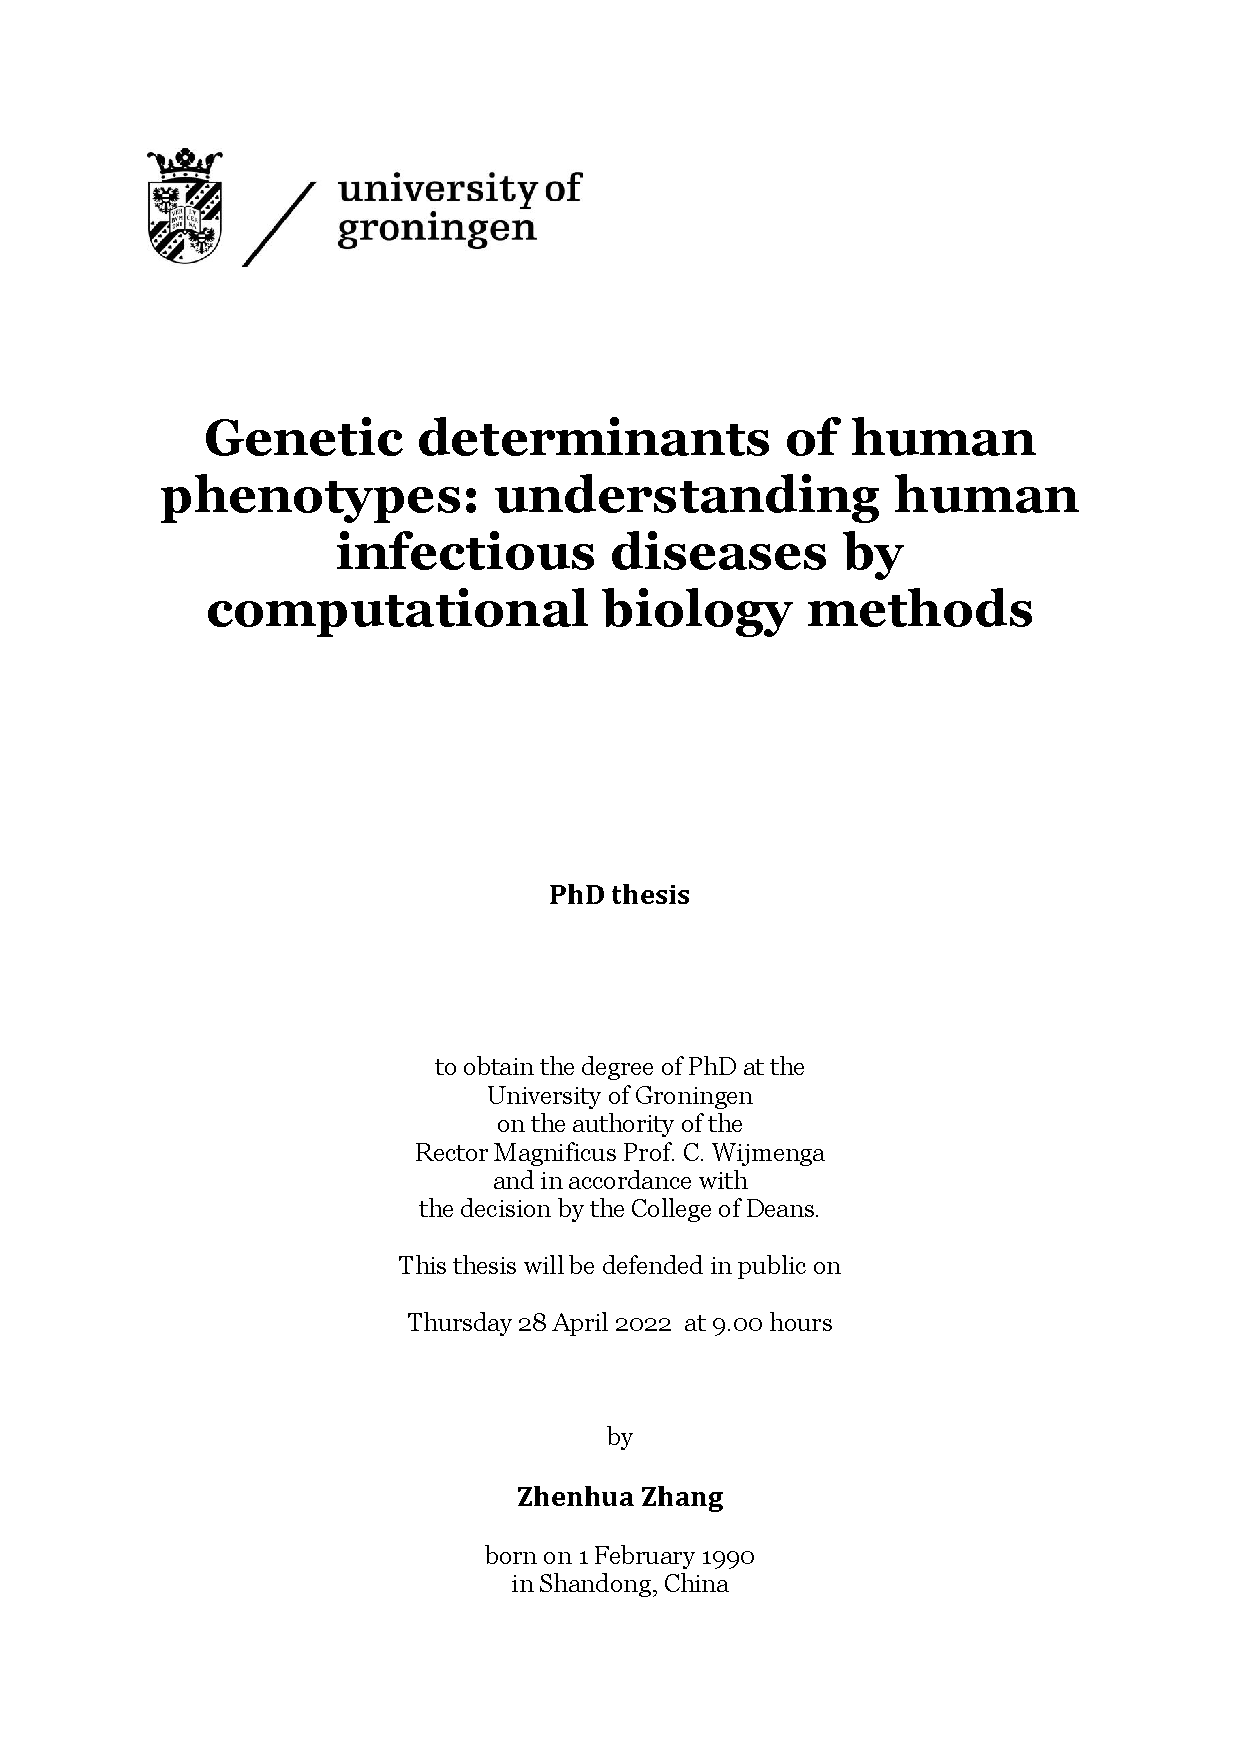
\includepdf[pages=1, trim=-12mm 0mm 0mm 0mm, clip]{src/rug-title-page.pdf}
\includepdf[pages=2, trim=0mm 25mm 0mm 25mm, clip]{src/rug-title-page.pdf}


% ----------------------------------------------------------------------------
% TOC
% ----------------------------------------------------------------------------
\tableofcontents
\clearpage


% ----------------------------------------------------------------------------
% Propositions
% ----------------------------------------------------------------------------
%\import{src/chapters/}{zzhang_phd-thesis_prepositions}


% ----------------------------------------------------------------------------
% Chapter 1 General introduction
% ----------------------------------------------------------------------------
\import{src/chapters/}{zzhang_phd-thesis_chapter1_general}


% ----------------------------------------------------------------------------
% Chapter 2
% ----------------------------------------------------------------------------
\import{src/chapters/}{zzhang_phd-thesis_chapter2_feasibility}


% ----------------------------------------------------------------------------
% Chapter 3
% ----------------------------------------------------------------------------
\import{src/chapters/}{zzhang_phd-thesis_chapter3_asdeep}


% ----------------------------------------------------------------------------
% Chapter 4
% ----------------------------------------------------------------------------
\import{src/chapters/}{zzhang_phd-thesis_chapter4_irf7}


% ----------------------------------------------------------------------------
% Chapter 5
% ----------------------------------------------------------------------------
\import{src/chapters/}{zzhang_phd-thesis_chapter5_ccr5}


% ----------------------------------------------------------------------------
% Chapter 6
% ----------------------------------------------------------------------------
\import{src/chapters/}{zzhang_phd-thesis_chapter6_single-cell}


% ----------------------------------------------------------------------------
% Chapter 7
% ----------------------------------------------------------------------------
\import{src/chapters/}{zzhang_phd-thesis_chapter7_discussion}


% ----------------------------------------------------------------------------
% Appendices
% ----------------------------------------------------------------------------
\import{src/chapters/}{zzhang_phd-thesis_appendix}


% ----------------------------------------------------------------------------
% Short summary
% ----------------------------------------------------------------------------
% \import{src/chapters/}{zzhang_phd-thesis_short-summary}


\end{document}
% vim: set tw=500:
